\documentclass[UTF8]{article}
\usepackage{ctex}
\usepackage{amssymb}
\usepackage{caption}
\usepackage{algorithmicx}
\usepackage{algorithm}
\usepackage{cite}
\usepackage{natbib}
\usepackage{amsmath}
\usepackage{float}
\usepackage{algpseudocode}  
\usepackage{graphicx, subfig}
\pagestyle{headings}
\begin{document}
\author{李奡程 161220062}
\title{并行计算项目报告}
\maketitle
\section{综述}
排序是一个历史悠久的问题,简单来说其要求对于输入序列$a_1,a_2,\ldots,a_n$,按照某一特定顺序将其输出。人们已经研究出了多种不同的排序手段,例如插入排序、冒泡排序、归并排序、快速排序、枚举排序、堆排序、基数排序等,而且人们已经证明基于比较的排序算法运行时间下界为$\omega(n\log n)$,所以在目前的时代采用并行化提高算法效率成为可选之举。
\par 在本次实验中,我用$C\#$实现了快速排序、归并排序和堆排序的串行版本和并行版本,设计了和书本中不完全一样的算法流程,并对它们的性能进行分析。(注:在本次实验中,默认要求顺序为单调递增)
\section{串行算法原理简述}
\subsection{枚举排序}
枚举排序通过比较比一个元素$a_i$小的元素的个数来确定其应处在的排完序后的序列中的位置,其运行时间为$O(n*n)=O(n^2)$.
\subsection{归并排序}
归并排序采用分治的思想,即先将原序列分割成两个规模较小的子序列分别排序,然后将两个排好序后的子序列进行处理得到最后的结果,其运行时间递归式为$T(n)=2T(\frac{n}{2})+\Theta(n)$,使用主定理解得其运行时间为$\Theta(n\log n)$.
\subsection{快速排序}
快速排序也采用分治的思想,但它每一步进行划分的时候仅依靠主元将其分为两个子序列,并保证左子序列中的所有元素都不大于主元,而右子序列中的所有元素都不小于主元,从而完成划分。这种算法最坏情况下算法复杂度为$O(n^2)$,而其期望时间复杂度为$\Theta(n\log n)$,且其以关于$n$的高概率趋于$\Theta(n\log n)$.
\par 为了保证随机性,可以在选取主元的时候采取随机化的方法,减轻对于输入的依赖。
\section{并行枚举排序}
\subsection{算法设计}
由以上关于枚举排序的过程可见,其运行过程中需要对于每个元素统计小于它的元素的个数,而这个过程是可以分开进行的,相当易于并行化处理。按照上述思路,我设计了如下的流程,并用伪代码表示如下:
\begin{algorithm}
\caption{主处理器的并行枚举排序伪代码}	
\begin{algorithmic}[1]
\Require 数组$a_1,a_2,\ldots,a_n$,处理器数目$p$  
\Function {ParallelEnumerationSortMaster}{$a,p$}  
\State $rangeLength \gets \frac{n}{p}$  
\State Master prepares a common space $spareSpace$
\For {i in range($p$)}
\State $left \gets i*rangeLength$
\State $right \gets (i+1)*rangeLength$
\State Master call $p_i$ to do [$left$,$right$] on $spareSpace$
\EndFor
\State Master wait for all $p$ processors to finish
\State Master copies data from $spareSpace$ to $a$
\State \Return{$a$}  
\EndFunction 	
\end{algorithmic}
\end{algorithm}
其中主处理器负责分配任务(安排每个处理器的处理范围),分配备用空间以存放中间排序结果以及等待所有子处理器工作完成后将最终结果拷贝回原数组中,而从处理器负责进行处理范围中的枚举计数并将结果送到备用空间中的相应位置上。
\begin{algorithm}
\caption{从处理器的并行枚举排序伪代码}	
\begin{algorithmic}[1]
\Require 数组$a_1,a_2,\ldots,a_n$,处理范围$left$和$right$,排序结果存放地点$b$  
\Function {ParallelEnumerationSortWorker}{$a,left,right,b$}  
\State $rangeLength \gets \frac{n}{p}$  
\For {i in range($left,right$)}
\State $poz=\Call {CountNoBiggerThan}{a_i,a}$
\State $b[poz]=a_i$
\EndFor
\EndFunction
\end{algorithmic}
\end{algorithm}
\subsection{算法分析}
在以上过程中,主处理器除了最后拷贝数据需$O(n)$外只花费常数时间;而在从处理器运行中,其每个数都要进行$O(n)$的时间统计(即函数$CountNoBiggerThan$),而其范围为$O(\frac{n}{p})$,故总的时间为$O(n*\frac{n}{p})=O(\frac{n^2}{p})$.而各处理器并行处理,故总时间为$O(n^2/p)$.
\par 而归并排序的串行算法耗时易见为$O(n^2)$,所以这种简单的并行版本已经保证达到$p$的加速比。
\subsection{技术要点}
\paragraph{(1)线程模拟} 此次实现中我采用c-sharp中的Thread来模拟处理器,由于其只支持void function(object arg)类型作为其线程入口,传参时必须要打包成object类型后才能使用Thread来调用,同时需要ParameterizedStart来启动线程。而线程收到object类型参数时需要按照相反顺序解包才能调用,所以相应地写了一些接口函数。
\paragraph{(2)同步} 以上算法主处理器中要求等待所有子处理器完成后再将结果拷贝到备用空间里(也即为排序结束),这里要求线程之间的同步。在我的实现中,我采用了c-sharp提供的Semaphore(信号量),用信号量的PV操作来完成,具体为在主线程中创建一个最大值为p的信号量\textbf{Semaphore s=new Semaphore(0,p);},然后子线程完成任务时释放信号量\textbf{s.Release();},主线程在进行拷贝前需\textbf{for (i=0;i$<$p;i++) s.WaitOne();},通过以上三步保证主子线程间的同步。
\section{并行归并排序}
\subsection{算法设计}
归并排序中将原序列分成若干个子序列的过程先天的就可以并行进行,但是问题是并行后的merge部分,如果仍然使用主处理器单机处理,则耗时仍为$O(n)$,递归表达式为$T(n)=T(\frac{n}{p})+O(n)$,根据主定理其总的时间复杂度仍未$O(n\log n)$。所以,我们必须要想办法将merge的部分的时间复杂度也降下来。在本次实验中,我们采用书本上的正则采样方法进行并行的merge,其相应伪代码如下:\\
\begin{algorithm}
	\caption{正则采样归并排序流程}	
	\begin{algorithmic}[1]
		\Require 数组$a_1,a_2,\ldots,a_n$,处理器数目$p$  
		\Function {ParallelMergeSort}{$a,p$}  
		\State (1) 均匀划分:主处理器将n个元素均匀地划分成p段,每台处理器有$n/p$个元素;
		\State (2) 局部排序及采样:各从处理器使用串行排序算法对其负责的$n/p$个数进行排序,并正则采样出$p$个元素送回主处理器;
		\State (3) 选择主元:主处理器收到从$p$个处理器的$p^2$个数后进行排序,从里面选取$p-1$个数作为主元,并广播给所有从处理器;
		\State (4) 划分及交换:从处理器收到主元后将其段上的数据分成$p$段,并将第$i$段送到处理器$p_i$处;
		\State (5) 归并排序: 各处理器将交换好的数据进行归并排序,形成最后结果。
		\State \Return 数组$a$
		\EndFunction
	\end{algorithmic}
\end{algorithm}
在此流程中,通过正则采样,各处理器能将其负责的数据较为均匀地划分成$p$段,并且通过全局交换实际上已经完成了merge的过程,之后只需对各小段进行排序即可;而各小段是部分有序的数列,对这种部分有序的数列实际上存在更高效的排序方法。
\subsection{算法分析}
易见算法第一步和第二步在各个从处理器上耗时$O(\frac{n}{p}\log\frac{n}{p})$;第二三步中主处理器上挑选主元耗时$O(p+p^2\log p^2)=O(p^2\log p)$;第四步划分和交换在各个从处理器上耗时$O(n/p)$;第五步耗时$O(\frac{n}{p}\log\frac{n}{p})$。故累加可得该流程总时长为$O(\frac{n}{p}\log\frac{n}{p}+p^2\log p)$。
\par 当$p<<n$时,主要耗时还是花在各个处理器的排序上,此时其能达到近似为$p$的加速比;当$p=\Theta(n)$时,可以考虑将第三步中选择主元的过程也并行化,来保证$p$的加速比。
\subsection{技术要点}
\paragraph{(1)通信} 在这个流程中,虽然其有效实现了并行化的merge,但是其相应地增加了通信开销,比如主从处理器间和各从处理期间需要频繁通信,包括主元的选择与广播、划分后的全局交换。由于在本机上实现,所以我使用一个公共二维数组commonArea((p+1)*p)来记录主从之间的通信,相应的维数为对应的通信渠道。
\par 另外划分与交换我通过各子线程通过从主线程处获得的坐标信息直接将元素拷贝到备用空间的相应坐标位置处,同步后再从备用空间拷贝回各自的子空间上进行,这样避免了用Thread实现子线程之间的通信,而成为主从之间的双向通信。
\paragraph{(2)同步}由于此处需要主线程和子线程之间的双向联系,所以我们采用两个信号量c和s,在需要等待的时候就使用\textbf{x.WaitOne()},完成工作时即发送信号\textbf{x.Release()},从而保证主从间的同步及结果正确。
\subsection{优化}
上述正则采样归并排序大部分运算过程(每个子处理器上的排序)并没有优化空间,但是划分交换后的各个子处理器上的数据由于其为数个部分排好序的数组的连接,可以考虑维护一个最小堆,每个元素为该串单调子列,每次从堆中取出最小元素进行排序,这样的话时间复杂度变为$O(\frac{n}{p}\log p)$,能够对原时间复杂度起到常数因子上的优化(因为子处理器中第一步中排序需时间$\Theta(\frac{n}{p}\log\frac{n}{p})$).
\section{并行快速排序}
\subsection{算法设计}
和归并排序类似,简单地将两个子序列并发执行并不能提高算法性能,必须将partition过程也改为并行进行。由于课本上构造二叉树需要$p=\Theta(n)$,这在$n$比较大的情况下并不现实,所以在这里我提出以下的并行划分算法:\\
\begin{algorithm}
	\caption{用于快排的并行划分过程}	
	\begin{algorithmic}[1]
		\Require 数组$a_1,a_2,\ldots,a_n$,处理器数目$p$
		\Ensure 主元位置$p$,且满足$(\forall i<p,p\geq a_i)\wedge(\forall i>p,p\leq a_i)$  
		\Function {ParallelPartition}{$a,p$}  
		\State (1) 均匀划分:主处理器选定主元$pivot$,将n个元素均匀地划分成p段,每台处理器有$n/p$个元素;
		\State (2) 局部统计:各从处理器统计在该段上比$pivot$小和大的元素的个数,并将其发给主处理器;
		\State (3) 划分分配:主处理器收到从$p$个处理器的元素个数信息,向各个处理器通知其将元素应送到的位置,并计算出$pivot$应处的位置$p$
		\State (4) 交换:子处理器将其段上的数据根据从主处理器接收的坐标信息发送到备用空间的对应位置;
		\State (5) 拷贝:主处理器检查所有子处理器都完成后发出信号,所有子处理器将其负责元素从备用空间上拷贝回原数组$a$
		\State \Return $p$
		\EndFunction
	\end{algorithmic}
\end{algorithm}
使用上述划分方法,可以很快构造出一颗快排树,具体代码如图 \ref{paraBSTBuild}所示。
\begin{figure}
	\includegraphics[width=1.0\textwidth]{parallelBstBuild.JPG}
	\caption{使用并行快排划分进行任务划分}
	\label{paraBSTBuild}
\end{figure} 
\subsection{算法分析}
原始的partition由于需要扫描每个元素至少一遍,所以时间复杂度为$O(n)$。在我提出的上述并行划分方法中,第二步局部统计耗时$O(n/p)$,第三步划分分配计算耗时$O(p)$,第四步交换在每个子处理器上耗时$O(n/p)$,第五步也耗时$O(n/p)$,故总的时长为$O(n/p+p)$,即当$p<<n$时加速比能达到$p$,当$p=\Theta(n)$时可通过将第三步划分分配也并行化达到相同的加速比。
\par 通过将划分改为并行划分,将快排的各个分支进行并行化也确实能够有效提高算法效率,应该能达到与归并排序类似的$O(\frac{n}{p}\log\frac{n}{p})$的期望运行时间。
\subsection{技术要点}
这一部分没有太多新的技术要点,但选取划分的程度等调参成为该部分的重点,因为快排蕴含了不太均匀的划分对并行化带来的损失问题(可能某一线程上由于主元的选取问题任务数较少,导致其较早完成后空等),所以个人在本机上调参的经验结果为须将线程数设置地略多于处理数数目,才能达到更好的可扩放性。
\subsection{优化}
\paragraph{(1)随机化} 快排的最坏时间复杂度出现在输入序列为一个已经排好序的的情况下,而在上述并行归并排序的第五步时获得的序列已经是部分排好序的,在这种情况下直接快排性能较差。我通过随机选取主元的方式避免了这一点,同时使得此算法的鲁棒性增强。
\paragraph{(2)尾递归} 串行快排(作为子进程)的另一个问题是划分不佳时其递归调用的栈深度过长,可能造成segmentation fault。在此我使用尾递归的方法一定程度上减轻了这一问题可能带来的影响,具体代码见图 2.
\begin{figure}
	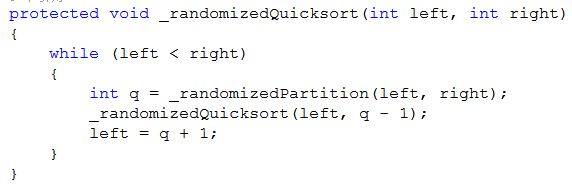
\includegraphics[width=1.0\textwidth]{tailRecursion.JPG}
	\caption{使用尾递归的快排}
	\label{tailRecursion}
\end{figure} 
\paragraph{(3)小规模时使用插入排序}当数据规模足够小时,使用分治算法带来的划分和merge的开销变得过大,这时可以考虑直接采用插入排序,减小递归深度且能提高运行效果(见SerialSortBase.cs中的\_randomizedImprovedQuicksort方法).
\section{性能分析}
\subsection{实验环境描述}
本次实验在Windows 10平台上进行,使用c\#语言用多线程模拟串行与并行排序算法,开发环境为Visual Studio 2013。此外,我使用c\#自带的System.Diagnostic中的Stopwatch类进行计时,并用Array.Sort方法作为系统库函数进行对比。
\par 另外,使用资源管理器发现本机有2个物理核,4个逻辑核,此为衡量并行化性能提升分析的参数。
\subsection{在给定数据集上的表现}
采用老师提供的random.txt数据集(数据类型为int,数据范围为$[-50000,50000]$,数据规模为30000),对该组数据运行10次取平均时间,我实现的六种算法表现如下:\\
\begin{table}
\centering
\begin{tabular}{|c|c|c|c|c|}
	\hline
	算法类型 & 枚举排序 & 归并排序 & 快速排序 & 库函数 \\
	\hline
	串行 & 12.5709 & 0.0106 & 0.00696 & 0.0029\\
	\hline
	并行 & 4.4911  & 0.00869 & 0.0103 & {}\\ 
	\hline
\end{tabular}
\caption{各排序算法在给定数据集上的表现}
\label{size30000}
\end{table} 
\\
另外,通过每次运行后对数据检查是否符合单调递增,可以检查排序算法实现的正确性,而在上述过程中所有的算法都正确运行。
\par 由表 \ref{size30000}结果可见,除了枚举排序有了明显的性能提升,归并排序的并行化并没有明显的提升,快排甚至有所下降。这是由于单机上创建线程与同步等造成的开销引起的,应该会随着输入规模的增加而减小。
\subsection{在不同规模数据集上的表现}
为了衡量算法的可扩放性,我将快排和归并的并串版本分别在不同规模的随机产生的数据集上运行10回合并计算平均时间,所得结果如下:(由于枚举排序复杂度太高,且性能较为稳定,所以在此不加入比较)\\
\begin{table}
\centering
\begin{tabular}{|c|c|c|c|c|}
	\hline
	数据规模 & $10^4$ & $10^5$ & $10^6$ & $10^7$ \\
	\hline
	串行归并排序 & 0.00391 & 0.0385 & 0.4735 & 4.888 \\
	\hline
	串行快速排序 & 0.00242 & 0.0276 & 0.3554 & 8.732 \\
	\hline
	并行归并排序 & 0.00424 & 0.0303 & 0.3651 & 3.856 \\
	\hline
	并行快速排序 & 0.00749 & 0.0290 & 0.2736 & 6.188 \\
	\hline
	库函数      & 0.00093 & 0.0104 & 0.1229 & 1.304 \\
	\hline
\end{tabular}
\caption{四种排序方法在不同规模数据集上的表现}
\label{differentScale}
\end{table} \\
\par 由表 \ref{differentScale}可见,并行归并算法在规模较大时性能较为稳定地超过其串行版本;而快排由于栈深度等问题,其在数据规模较大的时候出现了其他开销,导致性能反而有所下降,差于不用递归的归并排序。
\par 结合上述分析,可以看出采用并行化算法能够在数据集规模较大时显著提高算法性能,但是在单机上可能由于资源限制等问题出现别的损失,需根据机器配置和数据规模综合分析设计,选取适当的算法。
\begin{figure}
	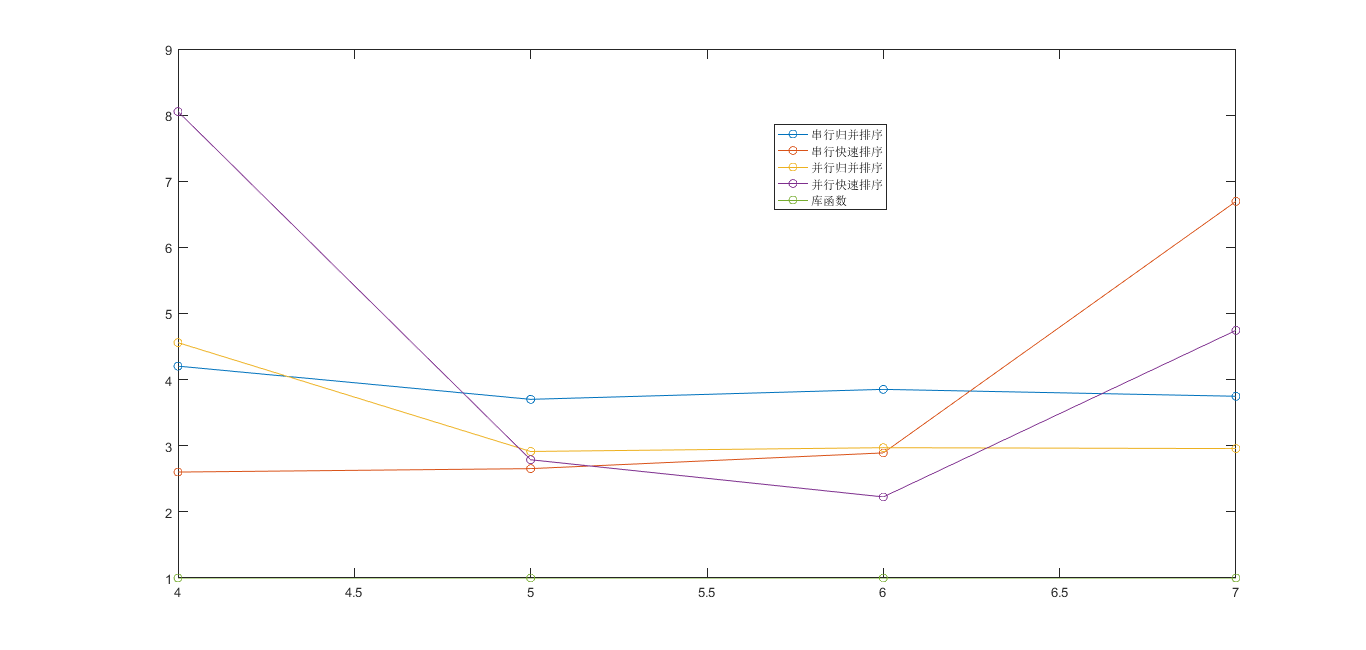
\includegraphics[width=1.0\textwidth]{growth.png}
	\caption{各排序算法时间与标准库对比}
	\label{finalComparison}
\end{figure} 
\section{总结}
在本次实验中,我使用c\#模拟实现了多种排序方法的串行和并行版本,并且提出了一种适用于快排的并行划分方法,其能够有效提高算法性能。此外我对其进行了在同一数据集和不同规模数据集上的实验,对其性能方面的提高与损失提出了解释。以后可以通过对于算法的进一步改进和并行化使其适应更大规模的数据,并且能够在更多处理器上并行处理。
\end{document}